\chapter{On Vectorial Leptoquarks Sensitivity at the LHC}

Leptoquarks ($\lq$s) are hypothetical bosons carrying both baryon and lepton number, thus interacting jointly with a lepton and a quark. They are a common ingredient in SM extensions where quarks and leptons share the same multiplet. Typical examples of these can be found in the Pati-Salam~\cite{Pati:1974yy} and $SU(5)$ GUT~\cite{Georgi:1974sy} models. In addition, they can also be found in theories with strong interactions, such as compositeness~\cite{Schrempp:1984nj}. Due to their exotic coupling which allows quark-lepton transitions, they have a diverse phenomenology, which naturally leads to several constraints. An important one comes from proton decay, which forces the $\lq$ mass to values close to the Planck scale, unless baryon and lepton numbers are not violated. Furthermore, in models where the latter are conserved, the $\lq$ can still be subject to a wide variety of bounds~\cite{Leurer:1993em,Davidson:1993qk,Leurer:1993qx,Hewett:1997ce,Queiroz:2014pra,Dorsner:2016wpm}. Examples of these come from meson mixing, electric and magnetic dipole moments, atomic parity violation tests, rare decays, and direct searches. Nevertheless, the significance of each bound is a model dependent question.
 
In the last years, an increased interest in low scale $\lq$s has emerged due to the anomalies in the precision measurements of the $\Bm$-meson decay rates. As it is well known, these corresponded mainly to deviations in the $R_{K^{(*)}}$~\cite{LHCb:2014vgu,LHCb:2017avl,LHCb:2019hip,LHCb:2021trn} and $R_{D^{(*)}}$~\cite{BaBar:2012obs,BaBar:2013mob,Abdesselam:2019dgh, Hirose:2017dxl, Sato:2016svk, Hirose:2016wfn, Huschle:2015rga,LHCb:2015gmp,Aaij:2015yra,Aaij:2017uff,LHCb:2017rln,LHCb:2023zxo} ratios, which measure the violation of lepton flavour universality (LFU). What followed was a very intense theoretical development, aiming to explain the anomalies by $\tev$ scale $\lq$ exchange at tree level~\cite{Hiller:2014yaa,Gripaios:2014tna,Alonso:2015sja,Calibbi:2015kma,Fajfer:2015ycq,Bauer:2015knc,Becirevic:2016oho,Crivellin:2017zlb,DAmico:2017mtc,Hiller:2017bzc,Buttazzo:2017ixm,Becirevic:2018afm,Cornella:2019hct,Angelescu:2021lln,Belanger:2021smw,GINO_2022}. Before the end of 2022, it was generally agreed that, within proposed single $\lq$ solutions, the only candidate capable of addressing all $\Bm$-meson anomalies simultaneously and surviving all other constraints was a vector $\lq$ ($U_1$), transforming as $({\bf 3},\,{\bf 1},\,2/3)$, and coupling mainly to third-generation fermions via $\bq\,\tau$ and $\tq\,\nu_\tau$ vertices~\cite{Buttazzo:2017ixm,Angelescu:2021lln}. In spite of a recent re-analysis of $R_{K^{(*)}}$ data showing this ratio to be compatible with the SM prediction~\cite{LHCb:2022qnv,LHCb:2022zom,Greljo:2022jac,Ciuchini:2022wbq}, the solution to the $R_{D^{(*)}}$ anomaly is still an open question and remains a valid motivation for the study of scenarios where new particles have preferential couplings to third-generation fermions. Thus, it is still of interest to continue exploring the possibility of observing the $U_1$ $\lq$ at the LHC~\cite{GINO_2022}. 

As expected, the theoretical community has extensively participated in probing $\lq$ models by scrutinizing search strategies, recasting LHC results, and predicting the reach in the parameter space via different searches involving third-generation fermions (see for instance~\cite{Diaz:2017lit,Dorsner:2018ynv,PhysRevD.99.035021,Schmaltz:2018nls,Biswas:2018snp,Baker:2019sli,Haisch:2020xjd,Bhaskar:2021gsy,Bernigaud:2021fwn,CompositenessGurrola}). In addition, several $13 \tev$ searches for $\lq$s decaying into $\tq/\bq$ and $\tau/\nu$ final states have been performed by the CMS~\cite{CMS:2016fxb,CMS:2017xcw,CMS:2018svy,CMS:2018qqq,CMS:2018txo,CMS:2018iye,CMS:2020wzx,CMS:2022goy,LQS_CMS_2022_results_comparison} and ATLAS~\cite{ATLAS:2019qpq,ATLAS:2020dsf,ATLAS:2021oiz,ATLAS:2021yij,ATLAS:2021jyv,ATLAS_7A,ATLAS_Vertical_Line} collaborations.

%Leptoquark Feynman Diagrams - fig:feynmp-prod-channels
\begin{figure}[!t]
    \centering
    %Single Leptoquark Production Diagram
    \begin{subfigure}[b]{0.45\textwidth}
        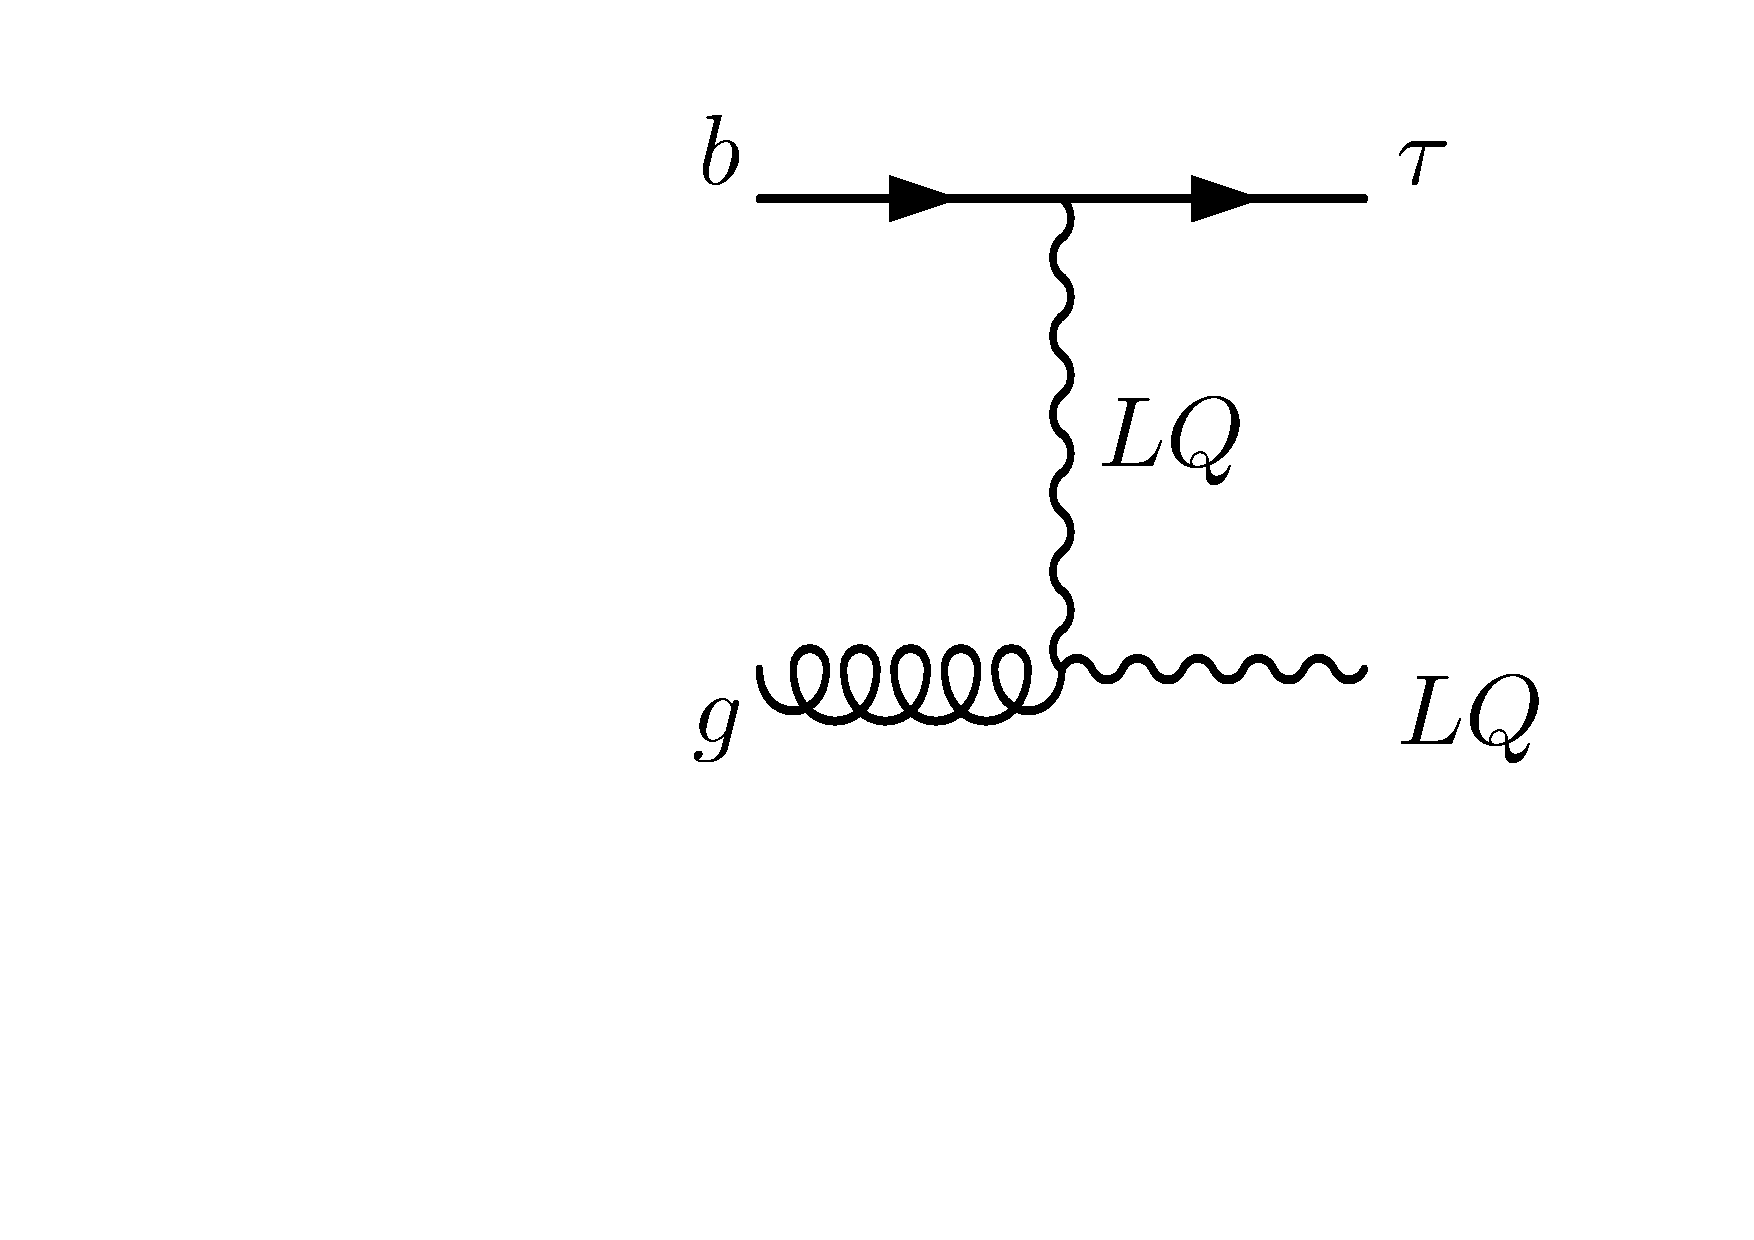
\includegraphics[width = 1.1\textwidth]{Images/feynman_diagrams/sLQ.pdf}
        \caption{}
    \end{subfigure}
    \hfill
    %Double Leptoquark Production Diagram
    \begin{subfigure}[b]{0.45\textwidth}
        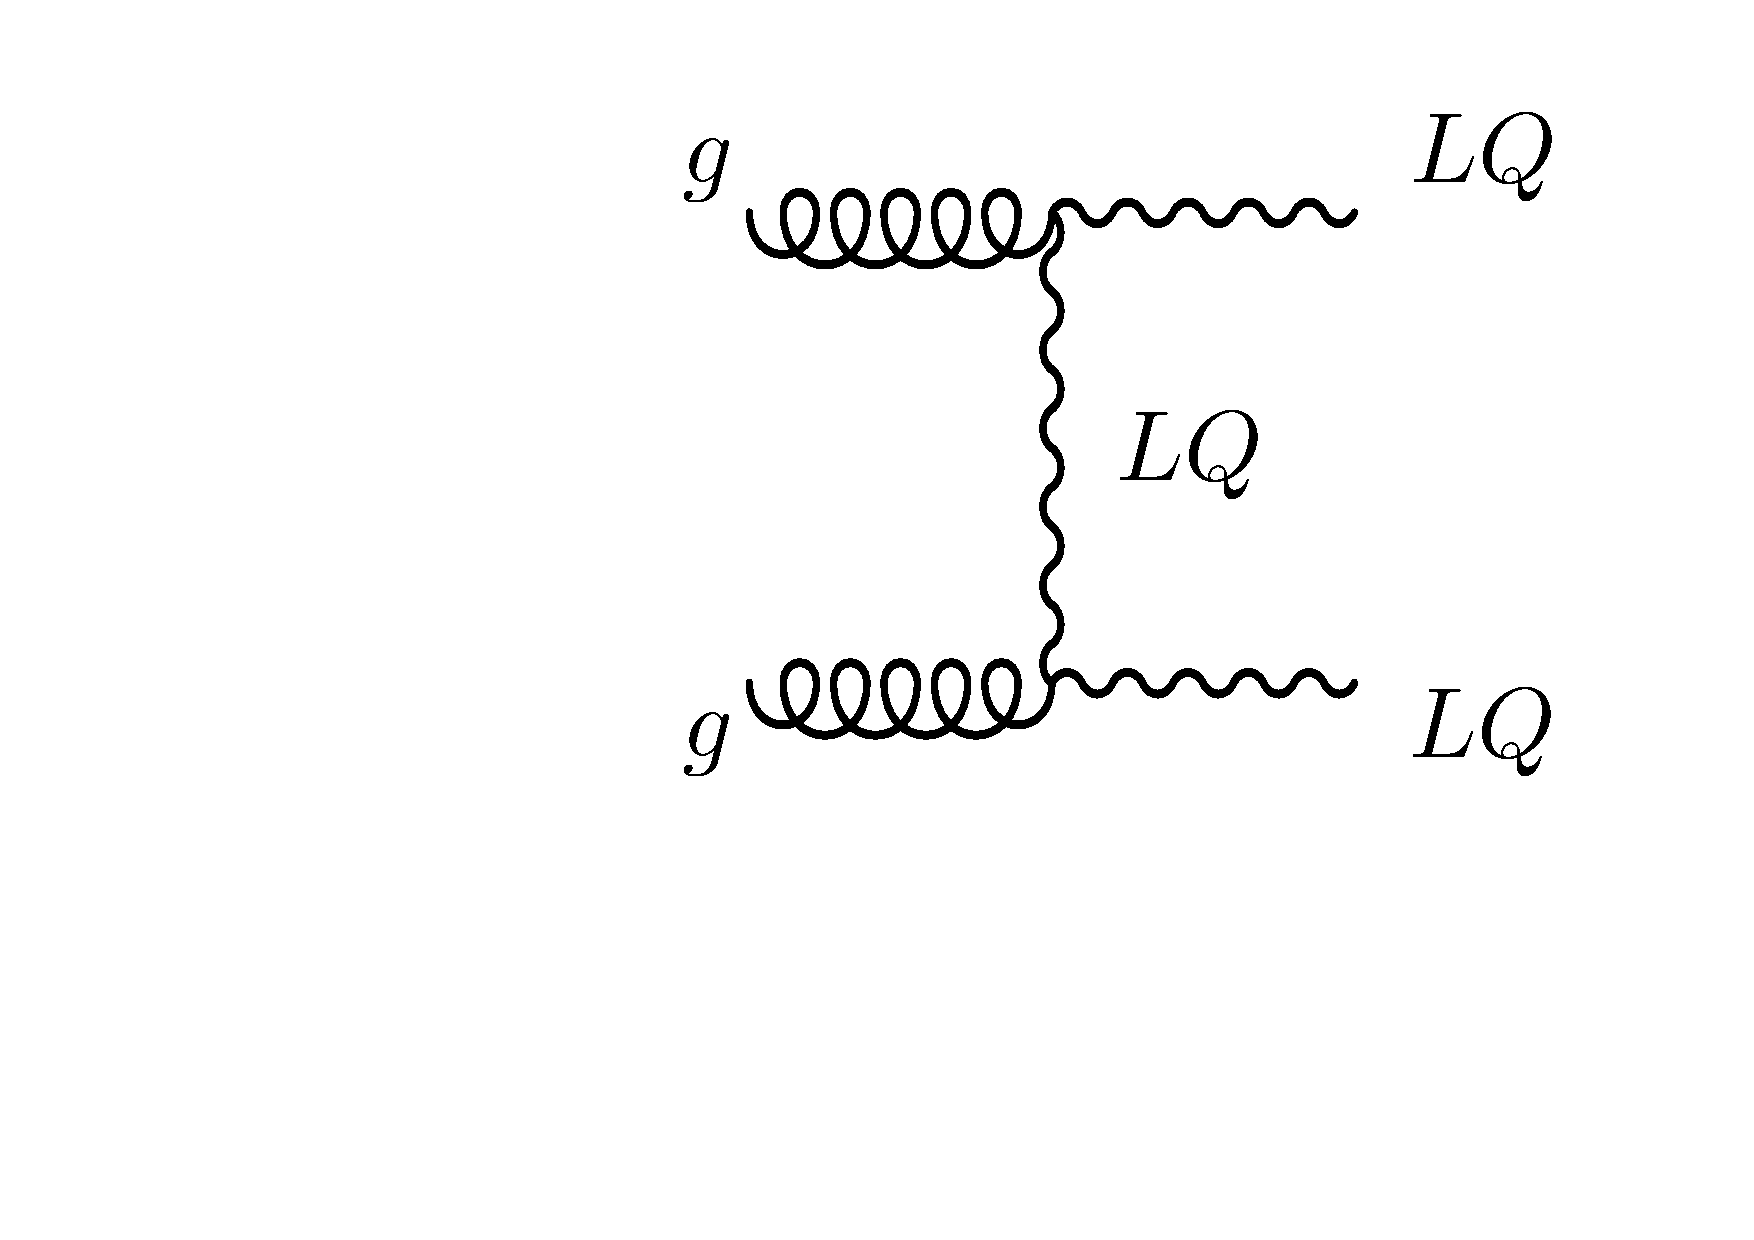
\includegraphics[width =  1.1\textwidth]{Images/feynman_diagrams/dLQ.pdf}
        \caption{}
    \end{subfigure}
    \hfill
    %non-resonant Leptoquark mediation Diagram
    \begin{subfigure}[b]{0.45\textwidth}
        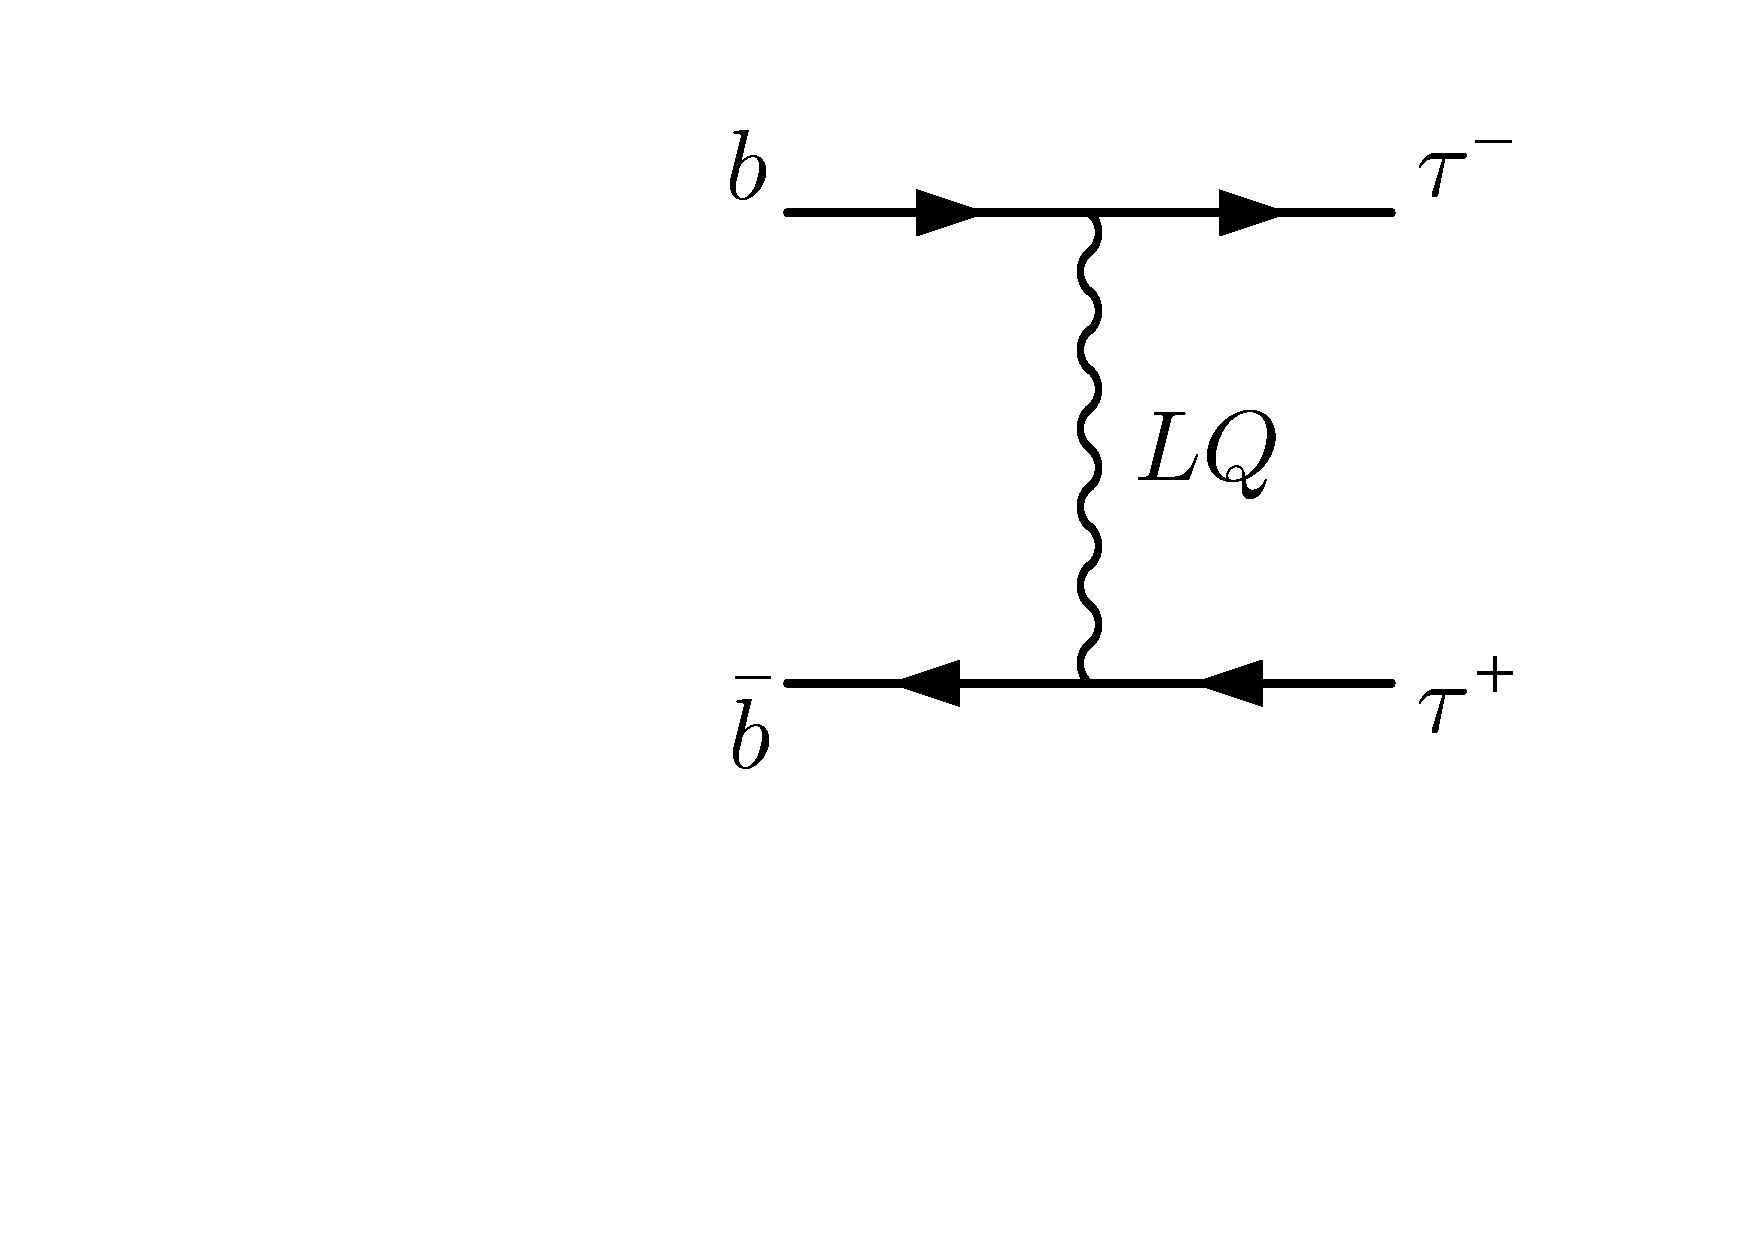
\includegraphics[width =  1.1\textwidth]{Images/feynman_diagrams/non_res.pdf}
        \caption{}
    \end{subfigure}
    \caption{Representative Feynman diagrams of single (a), pair  (b), and non-resonant (c) production leptoquarks in proton-proton collision experiments. In single and pair production, the diagrams shown involve t-channel LQ exchange, dominant for lower LQ mass. However, for larger mass there exist s-channel diagrams featuring a virtual bottom quark and gluon, respectively.}
    \label{fig:feynmp-prod-channels}
\end{figure}

Of the searches above, we find~\cite{CMS:2020wzx} particularly interesting. Here, the CMS collaboration explores signals corresponding to $\tq\,\nu\,\bq\,\tau$ and $\tq\,\nu\,\tau$ final states, with $137 \fb^{-1}$ of proton-proton ($\mathrm{p}\,\mathrm{p}$) collision data. The former is motivated by $\lq$ pair production, with one $\lq$ decaying into $\tq\,\nu$ and the other into $\bq\,\tau$, while the latter arises from a single $\lq$ produced in association with a $\tau$, with a subsequent $\lq$ decay into $\tq\,\nu$ (see Figure~\ref{fig:feynmp-prod-channels} for the corresponding diagrams). From the combination of both production channels, the search excludes $U_1$ masses under $1.3-1.7 \tev$, with this range depending on the $U_1$ coupling to gluons and on its coupling $g_U$ in the $\bq_L\,\tau_L$ vertex.

What makes this search particularly attractive is that, for the first time, an LHC collaboration directly places (mass dependent) bounds on $g_U$. This is important, since having information on this parameter is crucial in order to understand if the $U_1$ is really responsible for the $R_{D^{(*)}}$ anomaly. The inclusion of the single-$\lq$ production mode is important, since its cross-section is directly proportional to $g^2_U$. However, as can be seen in Figure~6 of~\cite{CMS:2020wzx}, the current constraints are dominated by pair production, with single-$\lq$ production playing a subleading role. While this is expected~\cite{Schmaltz:2018nls}, it still leads us to ponder the possibility of improving the sensitivity of LHC searches to single-$\lq$ production, and thus on achieving better constraints on $g_U$. Other complementary and similar searches to~\cite{CMS:2020wzx} were carried out by both ATLAS~\cite{ATLAS_7A} and CMS~\cite{LQS_CMS_2022_results_comparison}.

It is also well known, though, that searches for an excess in the high-$\pt$ tails of $\tau$ lepton distributions can strongly probe $g_U$, up to very large $\lq$ masses. Indeed, as shown in~\cite{Faroughy:2016osc,GINO_2022}, the new physics effective operators contributing to $R_D{^{(*)}}$ also contribute to an enhancement in the $\mathrm{p}\,\mathrm{p}\to\tau\tau$ production rates. This has motivated a large number of recasts~\cite{Angelescu:2018tyl,Schmaltz:2018nls,Baker:2019sli,Bhaskar:2021pml,Angelescu:2021lln,Cornella:2021sby,Allwicher:2022gkm,Haisch:2022afh,GINO_2022}, as well as a CMS search explicitly providing constraints in terms of $U_1$~\cite{CMS:2022goy}. Nevertheless, it is important to note that for these $\mathrm{p}\,\mathrm{p}\to\tau\tau$ processes, the $\lq$ participates non-resonantly, so contributions to the $\mathrm{p}\,\mathrm{p}\to\tau\tau$ rates and kinematic distributions from non-LQ BSM diagrams containing possible virtual particles, such as a heavy neutral vector boson $\zb'$, could spoil a straightforward interpretation of any possible excess~\cite{Baker:2019sli}. Thus, it is also necessary to understand how the presence of other virtual particles can affect the sensitivity of an analysis probing $g_U$.

In this work we study the projected $\lq$ sensitivity at the LHC, considering already available $\mathrm{p}\,\mathrm{p}$ data as well as the expected amount of data to be acquired during the High-Luminosity LHC (HL-LHC) runs. We explore a proposed analysis strategy which utilizes a combination of single-, double-, and non-resonant-LQ production, targeting  final states with varying $\tau$-lepton and b-jet multiplicities. 
The studies are performed considering various benchmark scenarios for different $\lq$ masses and couplings, also taking into account distinct chiralities for the third-generation fermions in the $\lq$ vertex. We also assess the impact of a companion $\zb'$, which is typical of gauge models, in non-resonant $\lq$ probes, and find that interference effects can have a significant effect on the discovery reach. We consider this effect to be of high interest, given that non-resonant $\lq$ production can have the largest cross-section, and thus could be an important channel in terms of discovery potential.

An important aspect of this work is that the analysis strategy is developed using a machine learning (ML) algorithm based on Boosted Decision Trees (BDT)\cite{friedman_greedy_2001}. The output of the event classifier is used  to perform a profile-binned likelihood test to extract the overall signal significance for each model considered in the analysis. The advantage of using BDTs and other ML algorithms has been demonstrated in several experimental and phenomenological studies~\cite{Ai:2022qvs,Biswas:2018snp,ATLAS:2017fak,Chigusa:2022svv,Chung:2020ysf,Feng:2021eke,ttZprime}. In our studies, we find that the BDT algorithm gives sizeable improvement in signal significance.

\section{A Simplified Model for the $U_1$ Leptoquark}
\label{sec:model}

Extending the SM with a massive $U_1$ vector $\lq$ is not straightforward, as one has to ensure the renormalizability of the model. Most of the theoretical community has focused on extensions of the Pati-Salam (PS) models which avoid proton decay, such as the scenario found in~\cite{Assad:2017iib}. Other examples include PS models with vector-like fermions~\cite{Calibbi:2017qbu,Blanke:2018sro,Iguro:2021kdw}, the so-called 4321 models~\cite{DiLuzio:2017vat,Greljo:2018tuh,DiLuzio:2018zxy}, the twin PS$^2$ model~\cite{King:2021jeo,FernandezNavarro:2022gst}, the three-site PS$^3$ model~\cite{Bordone:2017bld,Bordone:2018nbg,Fuentes-Martin:2022xnb}, as well as composite PS models~\cite{Gripaios:2009dq,Barbieri:2016las,Barbieri:2017tuq}.

In what follows, we shall restrict ourselves to a simplified non-renormalizable lagrangian, understood to be embedded into a more complete model. The SM is thus extended by adding the following terms featuring the $U_1$ $\lq$:
\begin{eqnarray}
\label{eq:BasicLagrangian}
  \mathcal{L}_{U_1}&=&-\frac{1}{2}U^\dagger_{\mu\nu}U^{\mu\nu}+M_U^2\, U_{1\mu}^\dagger U_1^\mu \nonumber \\
 &&  -ig_s\,U_{1\mu}^\dagger\, T^a\, U_{1\nu}\, G^{a\mu\nu}\!\!-i\frac{2}{3}g'\,U^\dagger_{1\mu}U_{1\nu}B^{\mu\nu} \nonumber \\
 && +\frac{g_U}{\sqrt 2}[U_{1\mu}(\bar Q_3\,\gamma^\mu L_3+\beta_L^{s\tau}\,\bar Q_2\,\gamma^\mu L_3 \nonumber \\  && +\beta_{R}\,\bar b_{R}\,\gamma^\mu \tau_{R}) +{\rm h.c.}] 
\end{eqnarray}
where $U_{\mu\nu}\equiv\mathcal{D}_\mu U_{1\nu}-\mathcal{D}_\nu U_{1\mu}$, and $\mathcal{D}_\mu\equiv\partial_\mu+ig_s T^a G_\mu^a+i\tfrac{2}{3}g'B_\mu$. As evidenced by the second line above, we assume that the $\lq$ has a gauge origin \footnote{The couplings in the second line of Eq.~(\ref{eq:BasicLagrangian}) can be found in the literature as $g_s\to g_s(1-\kappa_U)$ and $g'\to g'(1-\tilde\kappa_U)$, in order to take into account the possibility of an underlying strong interaction.}.

The third and fourth lines in in Eq.~(\ref{eq:BasicLagrangian}) shows the $\lq$ interactions with SM fermions, with coupling $g_U$, which we have chosen as preferring the third generation~\footnote{Before the demise of the $R_{K^{(*)}}$ anomaly~\cite{LHCb:2022qnv,LHCb:2022zom,Greljo:2022jac,Ciuchini:2022wbq}, a $3\times3$ $\beta_L$ matrix would be used instead, with values fitted to solve all $\Bm$ meson anomalies.}. These are particularly relevant for the $\lq$ decay probabilities, as well as for the single-$\lq$ production cross-section. The $\beta_L^{s\tau}$ parameter, which is the $\lq \to s\tau$ coupling in the $\beta_L$ matrix (see footnote), is chosen to be equal to $0.2$, following the fit done in~\cite{Cornella:2021sby}, in order to simultaneously solve the $R_{D^{(*)}}$ anomaly and satisfy the $\mathrm{p}\,\mathrm{p}\to\tau^+\tau^-$ constraints. Although $\beta_L^{s\tau}$ technically alters the single-$\lq$ production cross-section and $\lq$ branching fractions, we have confirmed that a value of $\beta_L^{s\tau} = 0.2$ results in negligible impact on our collider results, and thus is ignored in our subsequent studies.

The $\lq$ right-handed coupling is modulated with respect to the left-handed one by the $\beta_R$ parameter. The choice of $\beta_R$ is important phenomenologically, as it affects the $\lq$ branching ratios \footnote{Having $\beta_L^{s\tau}$ different from zero also opens new decay channels. These, however, are either suppressed by $\beta_L^{s\tau}$ and powers of $\lambda_{\rm CKM}$. In any case, this effect would decrease ${\rm BR}(\lq \to \bq\,\tau)$ and ${\rm BR}(\lq \to \tq\,\nu)$ by less than $3\%$.}, as well as the single-$\lq$ production cross-section. To illustrate the former, Fig.~\ref{fig:branching_ratios} (top) shows the $\lq\to\textrm{b}\tau$ and $\lq\to\textrm{t}\nu$ branching ratios as functions of the $\lq$ mass, for two values of $\beta_R$. For large $\lq$ masses, we confirm that with $\beta_R = 0$ then ${\rm BR}(\lq \to \bq\,\tau) \approx {\rm BR}(\lq \to \tq\,\nu)\approx \tfrac{1}{2}$. However, for $\beta_R = -1$, as was chosen in~\cite{Cornella:2019hct}, the additional coupling adds a new term to the total amplitude, leading to ${\rm BR}(\lq\to \bq\,\tau) \approx \tfrac{2}{3}$. The increase in this branching ratio can thus weaken bounds from $\lq$ searches targeting decays into $\tq\,\nu$ final states, which motivates exploring the sensitivity in b$\tau$ final states exclusively. Note that although a ${\rm BR}(\lq\to \bq\,\tau) \approx 1$ scenario is possible by having the $\lq$ couple exclusively to right-handed currents (i.e, $g_U\to0$, but $g_U\beta_R\not=0$), it does not solve the observed anomalies in the $R_{D^{(*)}}$ ratios. Therefore, although some LHC searches assume ${\rm BR}(\lq\to \bq\,\tau) = 1$, we stress that in our studies we assume values of the model parameters and branching ratios that solve the $R_{D^{(*)}}$ ratios.
\begin{center}
    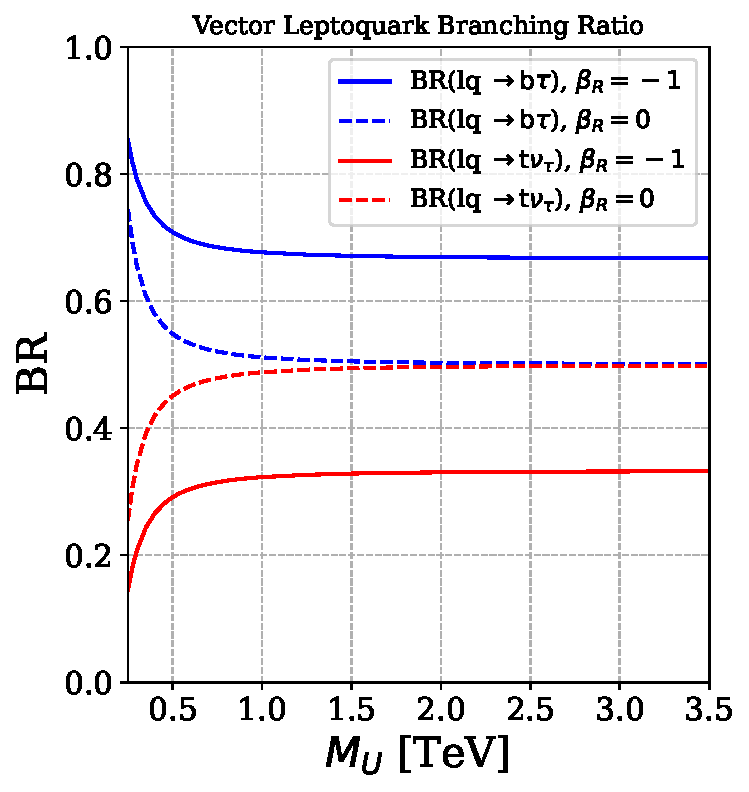
\includegraphics[width=.49\textwidth]{Images/VLQ_BranchingRatio.pdf}
    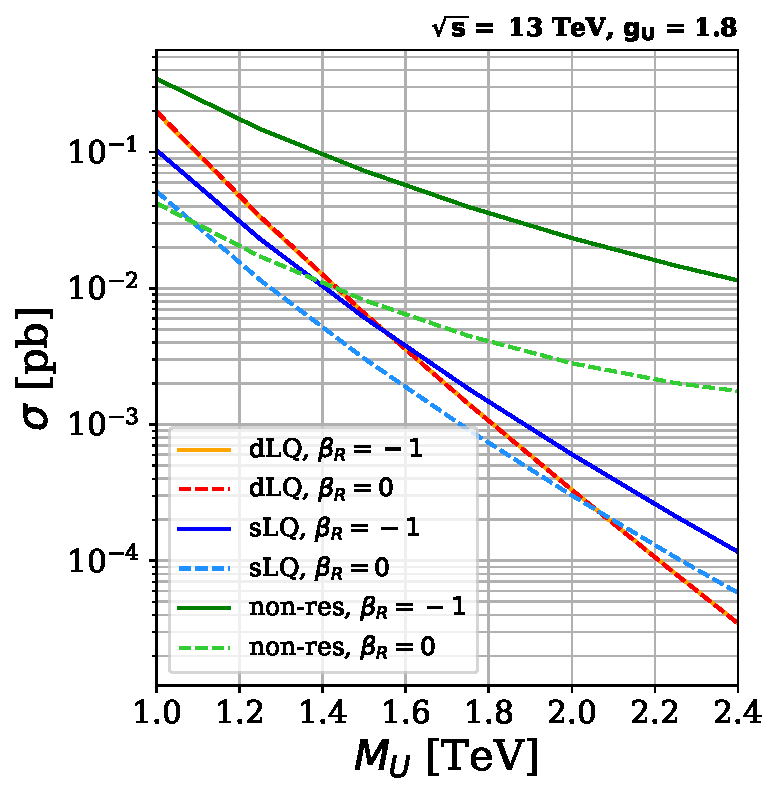
\includegraphics[width=.49\textwidth]{Images/prod_cross_section_13TeV.pdf}
    \captionof{figure}{Left: The $\lq\to\textrm{b}\tau$ and $\lq\to\textrm{t}\nu$ branching ratios for $\beta_{R} = 0$ (solid lines) and $\beta_{R} = -1$ (dashed lines). Right: Signal cross-section as a function of the $\lq$ mass, for $\sqrt{ s}=13 \tev$, with $g_U=1.8$. We show single, pair, and non-resonant production, for $\beta_R=-1,\,0$ in solid and dashed lines, respectively.}
\label{fig:branching_ratios}
\end{center}

To further understand the role of $\beta_R$ at colliders, Fig.~\ref{fig:branching_ratios} (bottom) shows the cross-section for single-$\lq$ (s$\lq$), double-$\lq$ (d$\lq$), and non-resonant (non-res) production, as a function of mass and for a fixed coupling $g_{U} = 1.8$, assuming $\mathrm{p}\,\mathrm{p}$ collisions at $\sqrt{s} = 13$ $\tev$. We note that this benchmark scenario with $g_{U}=1.8$ results in a $\lq\to\textrm{b}\tau$ decay width that is $<$5\% of the $\lq$ mass, for mass values from 250 $\gev$ to 2.5 $\tev$. In the Figure, we observe that, since d$\lq$ production is mainly mediated by events from quantum chromodynamic processes, the choice of $\beta_R$ does not affect the cross-section. However, for  s$\lq$ production, a non-zero value for $\beta_R$ increases the cross-section by about a factor of 2 and by almost one order of magnitude in the case of non-res production. These results shown in Fig.~\ref{fig:branching_ratios} are easily understood by considering the diagrams shown in Fig.~\ref{fig:feynmp-prod-channels}. The $\lq$ mass value where the s$\lq$ production cross-section exceeds the d$\lq$ cross-section depends on the choice of $g_U$. 
 
We also note that to solve the $R_{D^{(*)}}$ anomaly, the authors of~\cite{Cornella:2021sby} point out that the wilson coefficient $C_U\equiv g^2_U\,v^2_{SM}/(4\,M^2_U)$ is constrained to a specific range of values, and this range depends on the value of the $\beta_{R}$ parameter. Therefore, the allowed values of the coupling $g_{U}$ depend on $M_{U}$ and $\beta_{R}$, and thus our studies are performed in this multi-dimensional phase space.


We study the role of a $\zb'$ boson in $\mathrm{p}\,\mathrm{p}\to\tau\tau$ production. The presence of a $\zb'$ boson in $\lq$ models has been justified in various papers, for example, in~\cite{Baker:2019sli}. The argument is that minimal extensions of the SM which include a massive gauge $U_1$ LQ, uses the gauge group $SU(4)\times SU(3)^{\prime}\times SU(2)_L \times U(1)_{T_R^3}$. Such an extension implies the presence of an additional massive boson, $\zb^{\prime}$, and a color-octet vector, $G'$, arising from the spontaneous symmetry breaking into the SM, see for example App.~\cite{sec:4321}. \marginpar{Naively, the LQs are associated to the breaking of $SU(4)\to SU(3)_{[4]}\times U(1)_{B-L}$, the $G'$ arises from $SU(3)_{[4]}\times SU(3)'\to SU(3)_c$, and the $Z'$ comes from the breaking of $U(1)_{B-L}\times U(1)_{T_R^3}\to U(1)_Y$. Notice that the specific pattern of breaking, and the relations between the masses and couplings, are connected to the specific scalar potential used.}  The $\zb'$ in particular can play an important role in the projected $\lq$ discovery reach, as it can participate in $\mathrm{p}\,\mathrm{p}\to\tau\tau$ production by s-channel exchange, both resonantly and as a virtual mediator. To study the effect of a $\zb'$ on the $\mathrm{p}\,\mathrm{p}\to\tau\tau$ production cross-sections and kinematics, we extend our benchmark Lagrangian in Eq.~(\ref{eq:BasicLagrangian}) with further non-renormalizable terms involving the $\zb'$. Accordingly, we assume the $\zb'$ only couples to third-generation fermions. Our simplified model is thus extended by:
\begin{eqnarray}
    \label{eq:BasicLagrangianZp}
        \mathcal{L}_{Z^{\prime}}&= & -\frac{1}{4} Z_{\mu \nu}^{\prime} Z^{\prime \mu \nu}+\frac{1}{2} M_{Z^{\prime}}^2 Z_\mu^{\prime} Z^{\prime \mu} \nonumber \\
        && + \frac{g_{Z^{\prime}}}{2 \sqrt{6}} Z^{\prime \mu} (\zeta_q \bar{Q}_3 \gamma_\mu Q_3 \nonumber +\zeta_t \bar{t}_R \gamma_\mu t_R \\
        &&  +\zeta_b \bar{b}_R \gamma_\mu b_R-3 \zeta_{\ell} \bar{L}_3 \gamma_\mu L_3-3 \zeta_\tau \bar{\tau}_R \gamma_\mu \tau_R)
\end{eqnarray}
where the constants $M_{\zb^{\prime}}$, $g_{Z^{\prime}}$, $\zeta_q $, $\zeta_t $, $\zeta_b$, $\zeta_{\ell}$, $\zeta_\tau$, are model dependent.

We study two extreme cases for the $\zb'$ mass, following~\cite{GINO_PhysRevD.102.115015}, namely $M_{\zb'} = \sqrt{\tfrac{1}{2}}M_U<M_U$ and $M_{\zb'} = \sqrt{\tfrac{3}{2}}M_U>M_U$. We also assume the $\lq$ and $\zb'$ are uniquely coupled to left-handed currents, i.e. $\zeta_q=\zeta_\ell= 1$ and $\zeta_t=\zeta_b=\zeta_\tau=0$. With these definitions, Fig.~\ref{fig:xsinterference} shows the effect of the $\zb'$ on the $\tau\tau$ production cross-section, considering $g_U = 1$, $\beta_R=0$, and different $g_{\zb^{\prime}}$ couplings. On the left, the cross-sections corresponding to the cases where $M_{\zb'} = \sqrt{\tfrac{1}{2}}M_U$ are shown. As expected, the $\tau\tau$ production cross-section for the inclusive case (i.e., $g_{\zb'} \neq 0$) is larger than that for the $\lq$-only non-res process ($g_{\zb'} = 0$, depicted in blue). This effect increases with $g_{\zb'}$ and, within the evaluated values, can exceed the $\lq$-only cross-section by up to two orders of magnitude. In contrast, a more intricate behaviour can be seen on the right of Fig.~\ref{fig:xsinterference}, which corresponds to $M_{\zb'} = \sqrt{\tfrac{3}{2}}M_U$. Here, for low values of $M_U$, a similar increase in the cross-section is observed. However, for higher values of $M_U$, the inclusive $\mathrm{p}\,\mathrm{p}\to\tau\tau$ cross-section is smaller than the $\lq$-only $\tau\tau$ cross-section. This behaviour suggests the presence of a dominant destructive interference at high masses, leaving its imprint on the results.
\begin{center}
    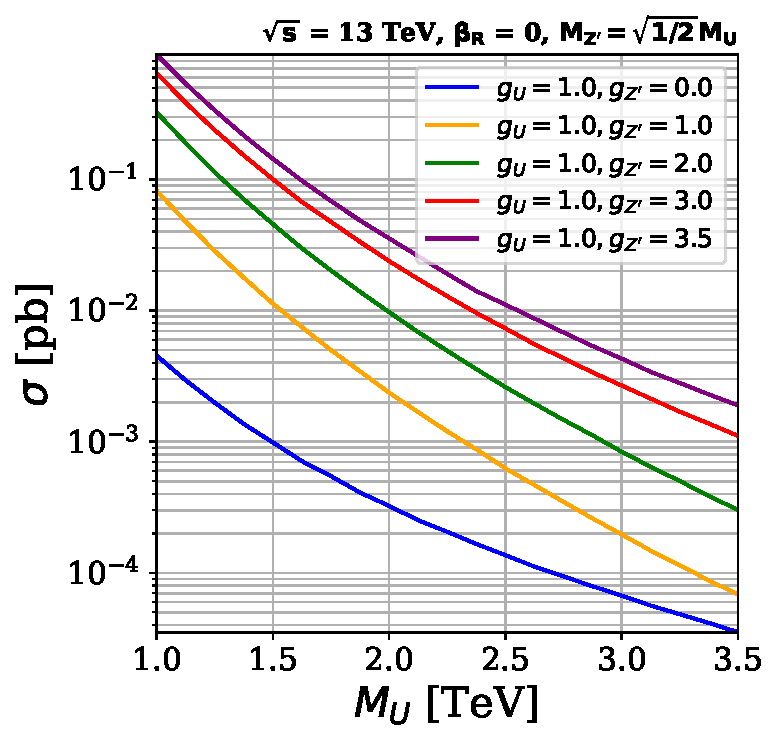
\includegraphics[width=.49\textwidth]{Images/XS_gu_gzp_lower_limit_woRHC.pdf}
    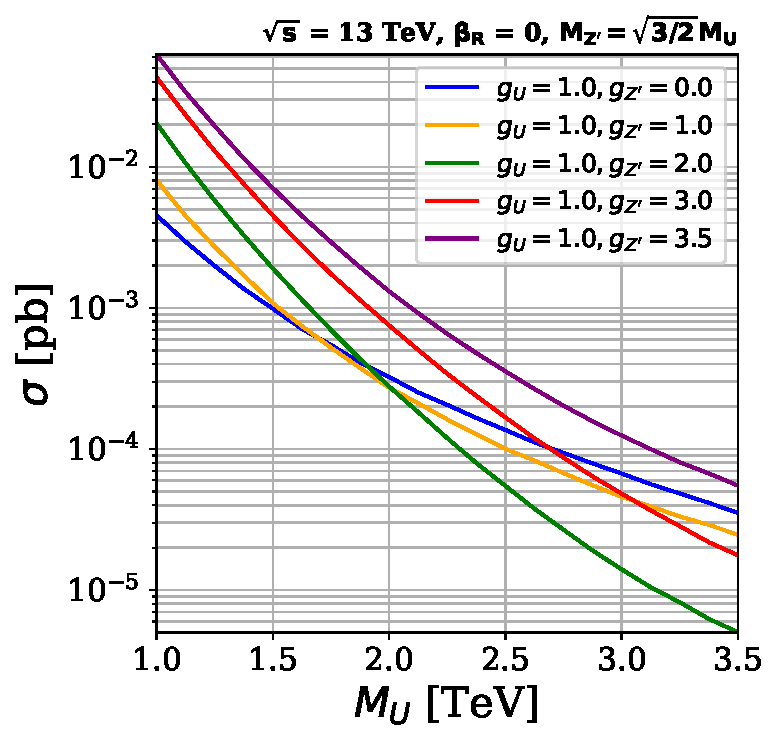
\includegraphics[width=.49\textwidth]{Images/XS_gu_gzp_upper_limit_woRHC.pdf}
    \captionof{figure}{$\tau \tau$ cross-section as a function of the $\lq$ mass for different values of $g_U$ and $g_{\zb^{\prime}}$. The estimates are performed at $\sqrt s=13 \tev$, $\beta_R=0$,  $M_{\zb^{\prime}} = \sqrt{1/2} M_{U}$ (left), and $M_{\zb^{\prime}} = \sqrt{3/2} M_{U}$ (right).}
\label{fig:xsinterference}
\end{center}

\begin{center}
    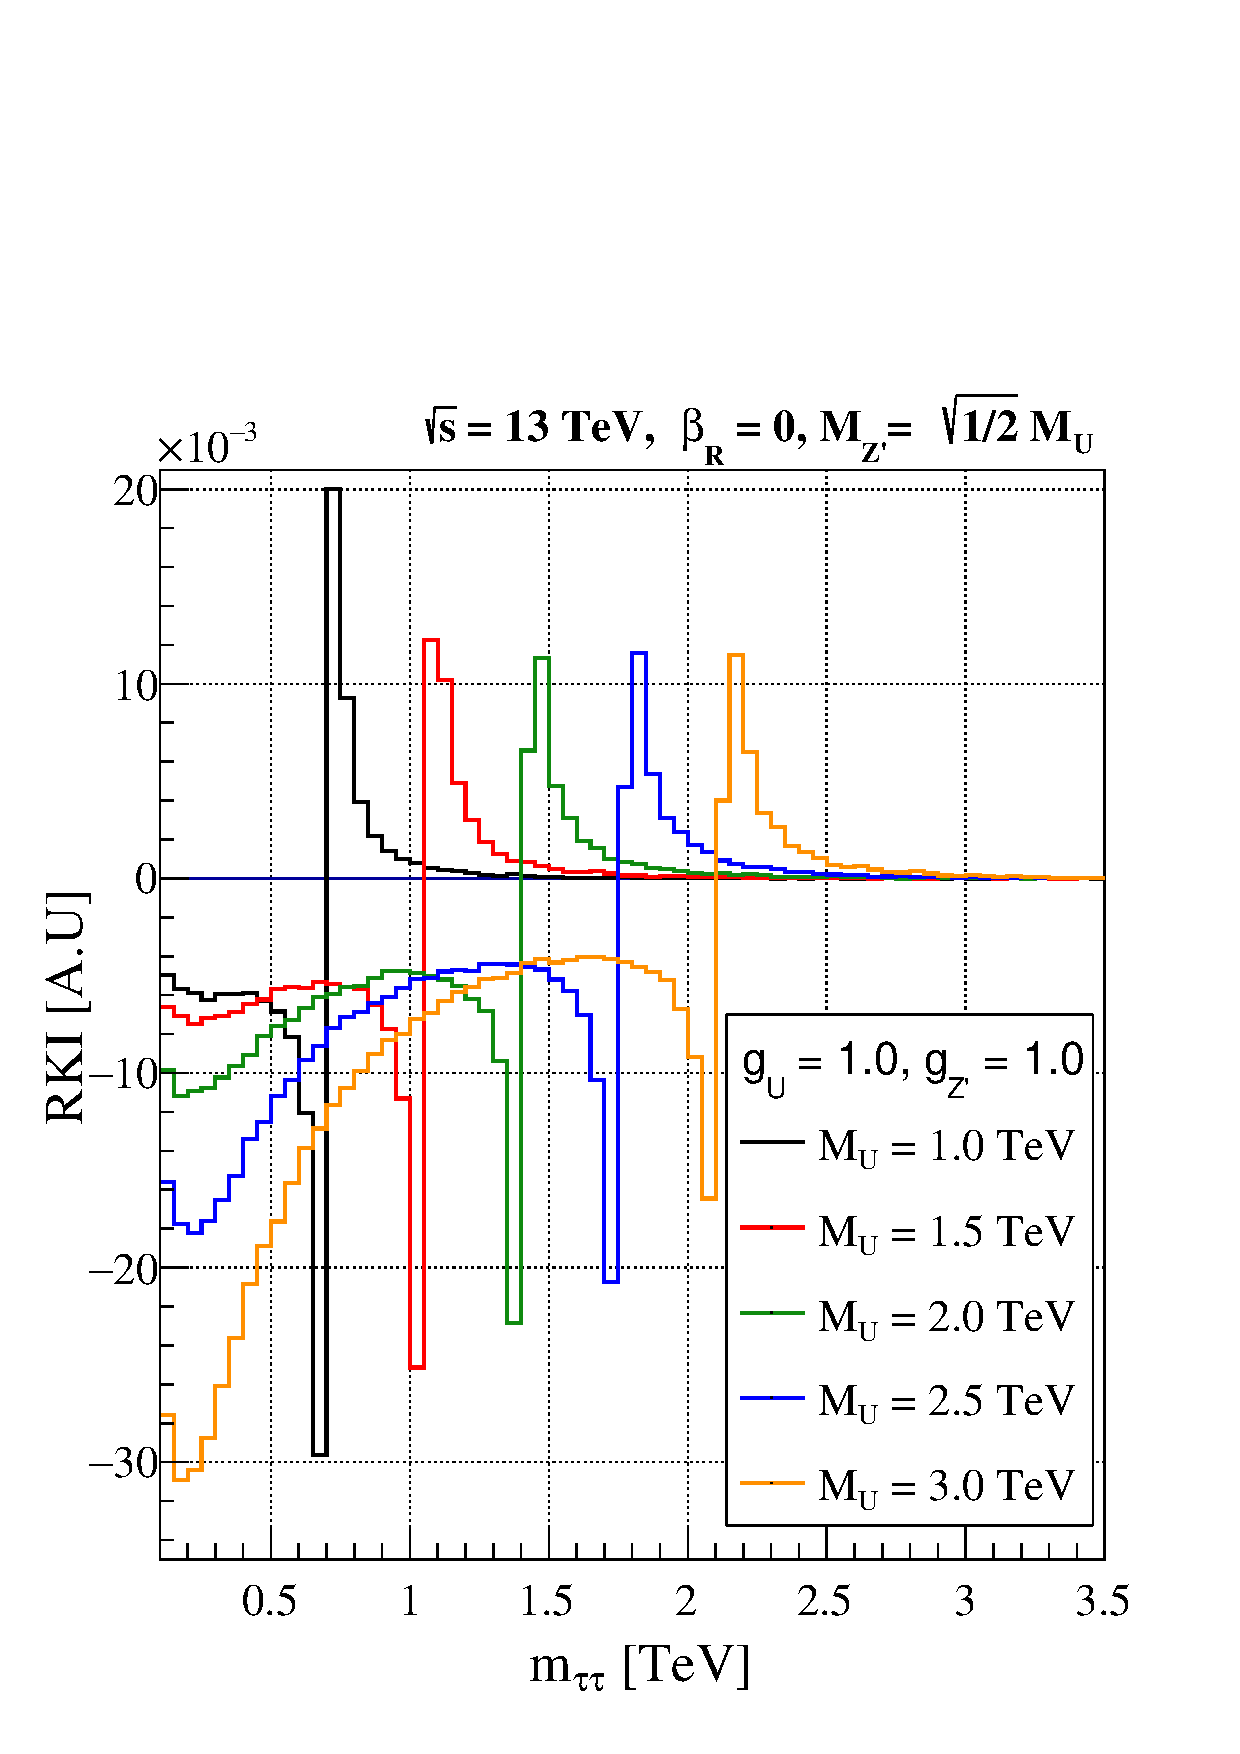
\includegraphics[width=.49\textwidth]{Images/Kinematic_Interference_gu_1.0_gzp_1.0_zp_lower_limit_woRHC.pdf}
    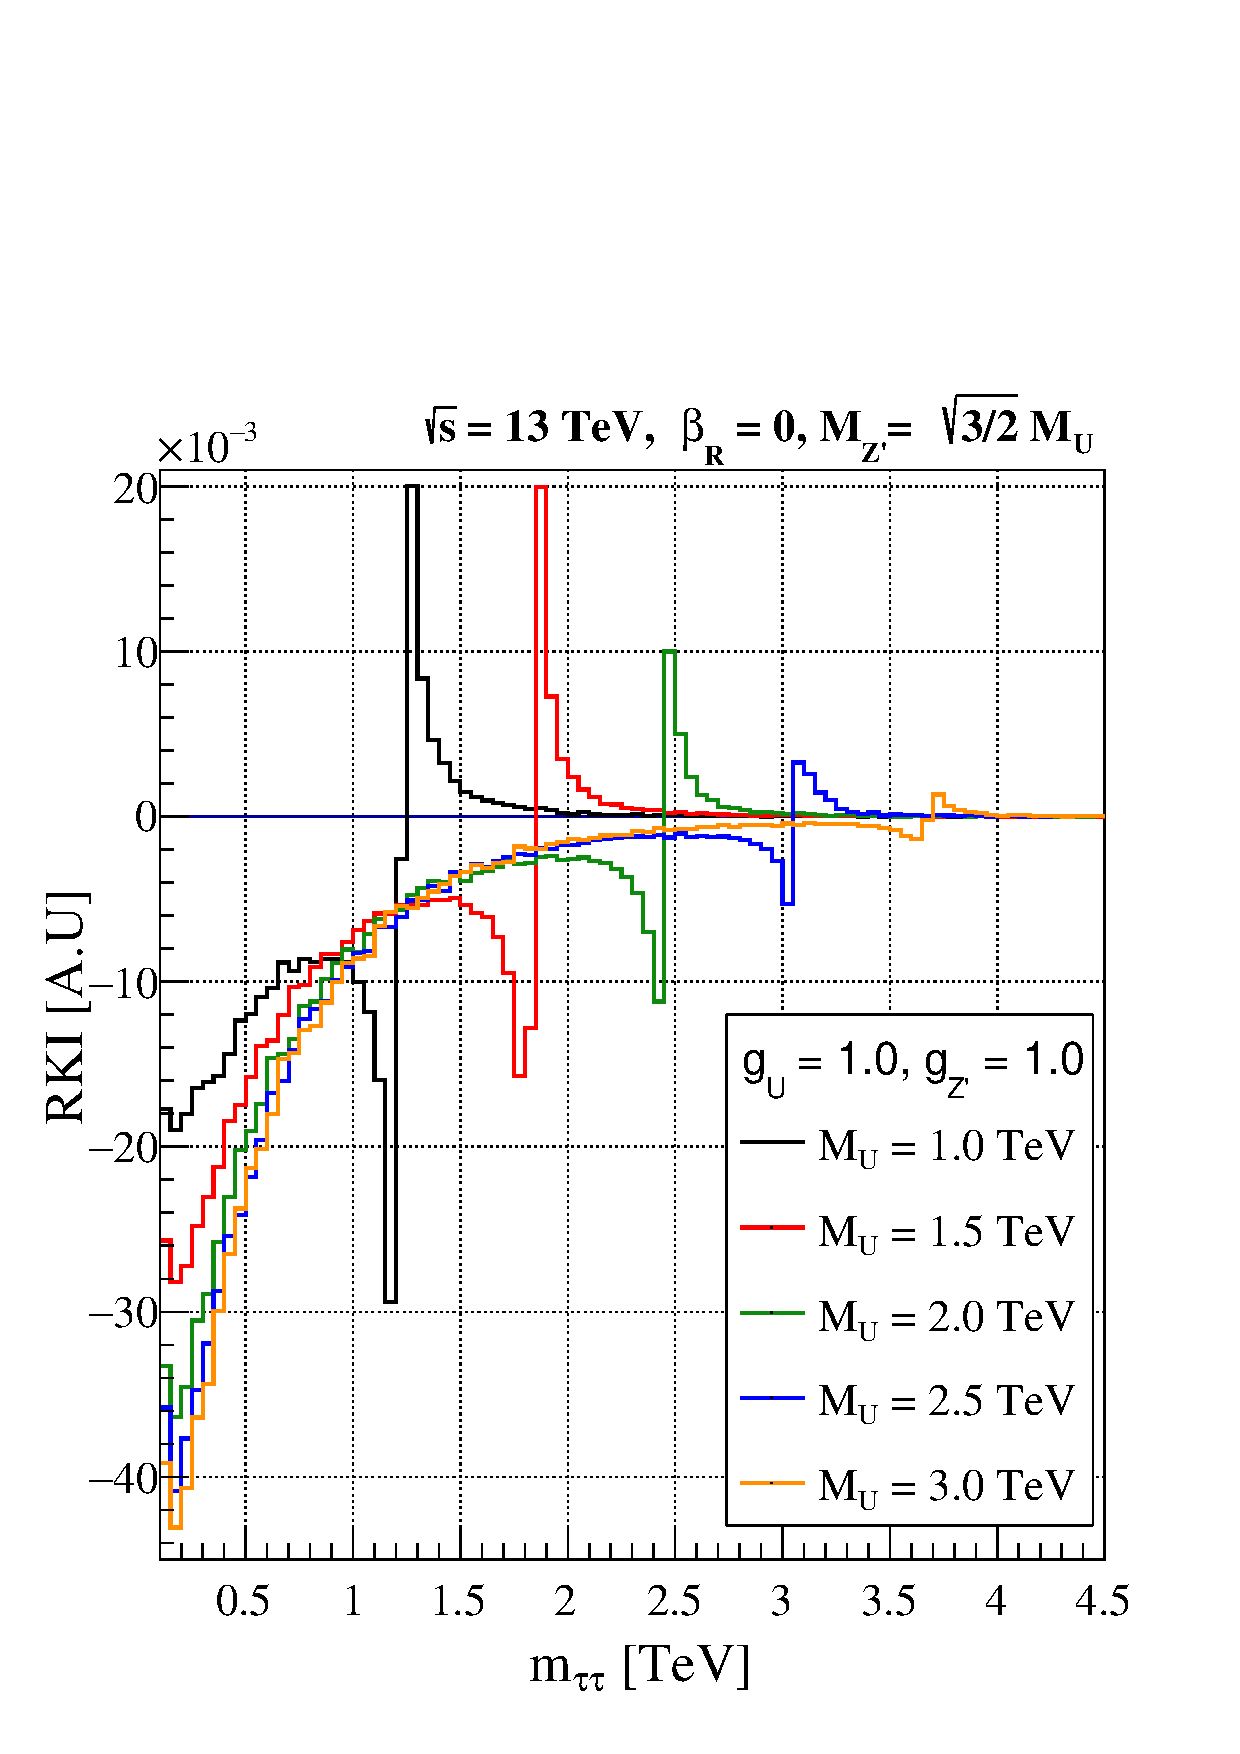
\includegraphics[width=.49\textwidth]{Images/Kinematic_Interference_gu_1.0_gzp_1.0_zp_upper_limit_woRHC.pdf}
    \captionof{figure}{The relative kinematic interference (RKI), as a function of the reconstructed mass of two taus, for different $\lq$ masses. The studies are performed assuming $\sqrt s=13 \tev$, $\beta_R=0$, $g_U = 1.0$, $g_{\zb^{\prime}} =1.0$, $M_{\zb^{\prime}} = \sqrt{1/2} M_{U}$ (left), and $M_{\zb^{\prime}} = \sqrt{3/2} M_{U}$ (right).
    }    
\label{fig:interference}
\end{center}
In order to further illustrate the effect, Fig.~\ref{fig:interference} shows the relative kinematic interference ($\mathrm{RKI}$) as a function of the reconstructed invariant mass $m_{\tau\tau}$, for $g_{\zb^{\prime}} = 1$ and varying values of $M_U$. The RKI parameter is defined as
\begin{equation}
    \mathrm{RKI}(m_{\tau\tau})=\frac{1}{\sigma_{\lq+\zb'}}\left[\frac{d\sigma_{\lq+\zb'}}{dm_{\tau\tau}}-\left(\frac{d\sigma_{\lq}}{dm_{\tau\tau}}+\frac{d\sigma_{\zb'}}{dm_{\tau\tau}}\right)\right],
\end{equation}
where $\sigma_{X}$ is the production cross-section arising due to contributions from $X$ particles. For example, $\sigma_{\lq+\zb'}$ represents the inclusive cross-section where both virtual $\lq$ and s-channel $\zb'$ exchange contribute. For both cases, we can observe the presence of deep valleys in the RKI curves when $m_{\tau\tau}\to0$, indicating destructive interference between the $\lq$ and the $\zb'$ contributions. This interference generates a suppression of the differential cross-section for lower values of $m_{\tau\tau}$ and, therefore, in the integrated cross-section. 
 
The observed interference effects are consistent with detailed studies on resonant and non-res $\mathrm{p}\,\mathrm{p}\to\tq \bar{\tq}$ production, performed in reference~\cite{Djouadi:2019cbm}.